\begin{frame}
	\titlepage
\end{frame}

\begin{frame}{\S\,5.5\;平面曲线的曲率}
	\linespread{1.5}
	\begin{enumerate}
	  \item {\bf 内容与要求}{\b( 教材上册P120-127 )}
	  \begin{itemize}
	    \item 理解曲率的概念
	    \item 熟练掌握曲率的计算公式
	    \item 了解曲率的应用
	  \vspace{1em}
	  \end{itemize}
	  \item {\bf 课后练习:}
	  \begin{itemize}
	    \item {\b 习题5.5:5,6,7,8,11}
	  \end{itemize}
	\end{enumerate}
\end{frame}

\begin{frame}{复习与回顾}
	\linespread{1.5}
	\ba{如何刻画一条平面曲线的几何特征?}
	
	\begin{enumerate}
	  \item {\bf 切线斜率:}一阶导数
	  \item {\bf 凹凸性:}二阶导数
	  \item {\bf 长度:}弧微分\pause
	  \item {\bf 弯曲程度:}{\b 曲率}
	\end{enumerate}
\end{frame}

%=================================================

\begin{frame}{曲率}
	\linespread{1.2}
	\centerline{\ba{如何刻画曲线的弯曲程度?}}
	\pause
	\begin{columns}
		\column{.5\textwidth}
			\begin{center}
				\vspace{-1em}
				{\resizebox{!}{5.5cm}{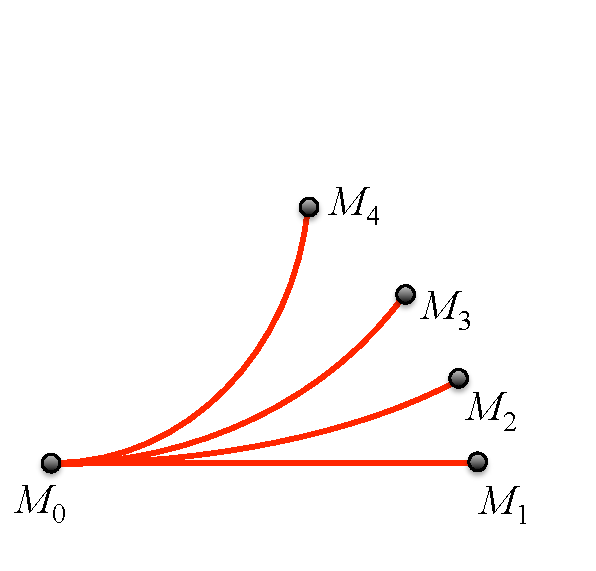
\includegraphics{./images/curves/c106.pdf}}}

				\vspace{-1em}\invisible<1->{{\b 长度相同的曲线,切线

				转角越大弯曲程度越大}}
			\end{center}
		\column{.5\textwidth}
	\end{columns}
\end{frame}

\begin{frame}{曲率}
	\linespread{1.2}
	\centerline{\ba{如何刻画曲线的弯曲程度?}}

	\begin{columns}
		\column{.5\textwidth}
			\begin{center}
				\vspace{-1em}
				{\resizebox{!}{5.5cm}{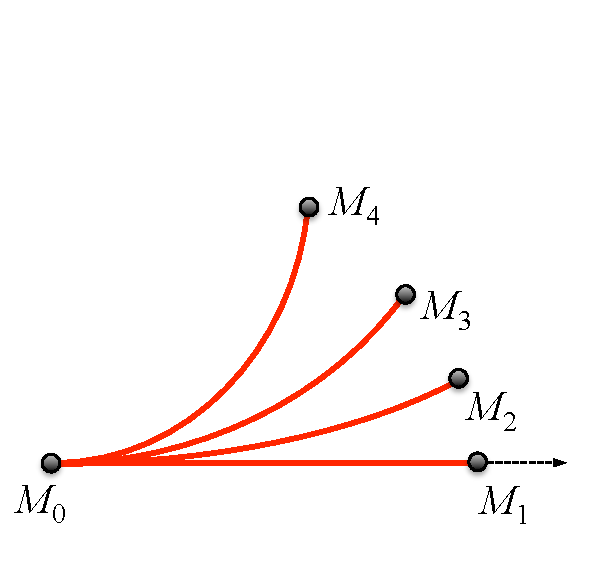
\includegraphics{./images/curves/c105.pdf}}}

				\vspace{-1em}\invisible<1->{{\b 长度相同的曲线,切线

				转角越大弯曲程度越大}}
			\end{center}
		\column{.5\textwidth}
	\end{columns}
\end{frame}

\begin{frame}{曲率}
	\linespread{1.2}
	\centerline{\ba{如何刻画曲线的弯曲程度?}}

	\begin{columns}
		\column{.5\textwidth}
			\begin{center}
				\vspace{-1em}
				{\resizebox{!}{5.5cm}{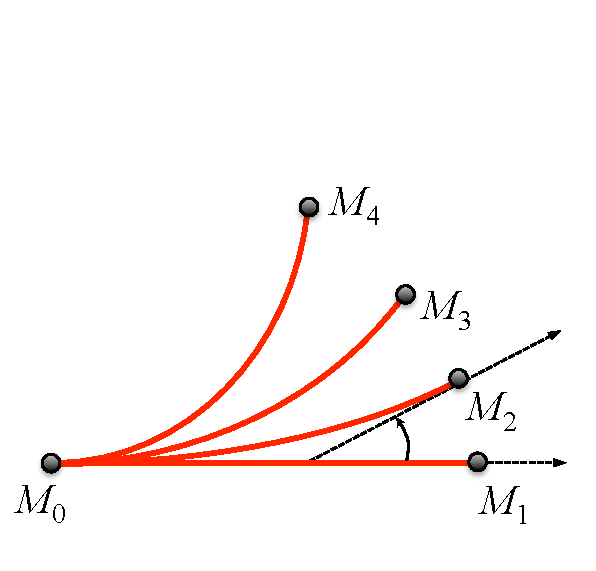
\includegraphics{./images/curves/c104.pdf}}}

				\vspace{-1em}\invisible<1->{{\b 长度相同的曲线,切线

				转角越大弯曲程度越大}}
			\end{center}
		\column{.5\textwidth}
	\end{columns}
\end{frame}

\begin{frame}{曲率}
	\linespread{1.2}
	\centerline{\ba{如何刻画曲线的弯曲程度?}}

	\begin{columns}
		\column{.5\textwidth}
			\begin{center}
				\vspace{-1em}
				{\resizebox{!}{5.5cm}{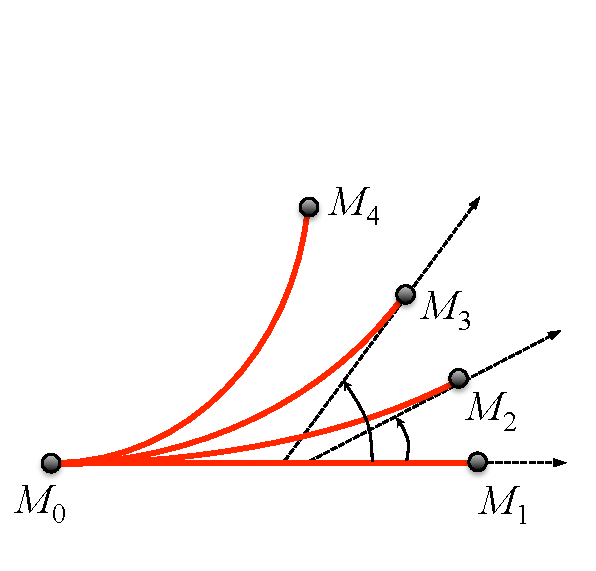
\includegraphics{./images/curves/c103.pdf}}}

				\vspace{-1em}\invisible<1->{{\b 长度相同的曲线,切线

				转角越大弯曲程度越大}}
			\end{center}
		\column{.5\textwidth}
	\end{columns}
\end{frame}

\begin{frame}{曲率}
	\linespread{1.2}
	\centerline{\ba{如何刻画曲线的弯曲程度?}}

	\begin{columns}
		\column{.5\textwidth}
			\begin{center}
				\vspace{-1em}
				{\resizebox{!}{5.5cm}{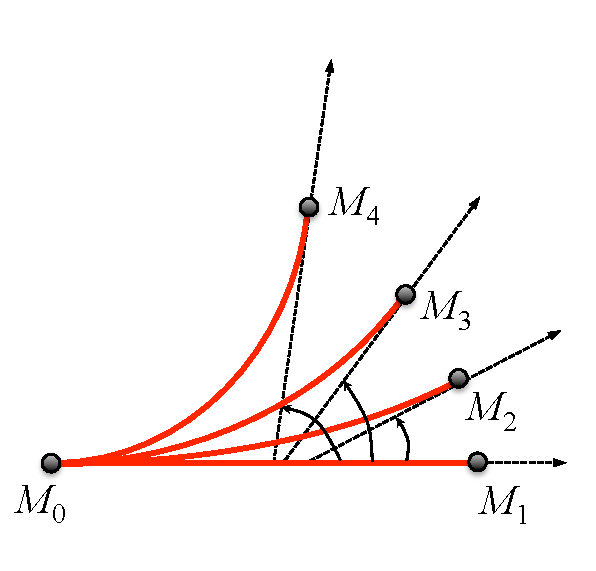
\includegraphics{./images/curves/c102.pdf}}}

				\vspace{-1em}\invisible<1->{{\b 长度相同的曲线,切线

				转角越大弯曲程度越大}}
			\end{center}
		\column{.5\textwidth}
	\end{columns}
\end{frame}

% \begin{frame}{曲率}
% 	\linespread{1.2}
% 	\centerline{\ba{如何刻画曲线的弯曲程度?}}
% 
% 	\begin{columns}
% 		\column{.5\textwidth}
% 			\begin{center}
% 				\vspace{-1em}
% 				{\resizebox{!}{5.5cm}{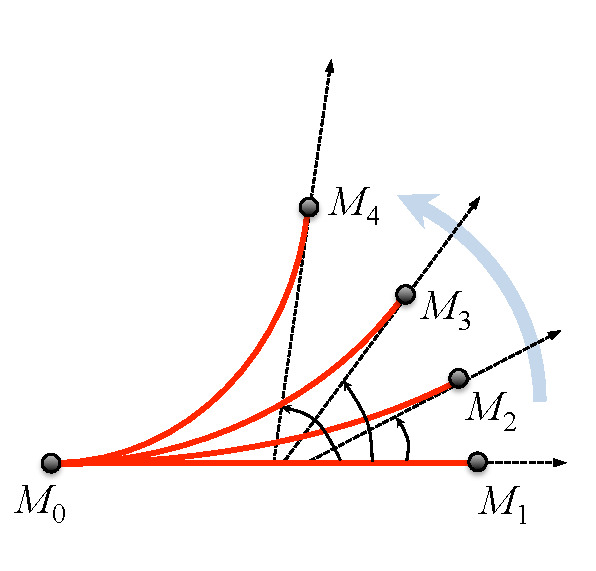
\includegraphics{./images/curves/c101.pdf}}}
% 
% 				\vspace{-1em}\invisible<1->{{\b 长度相同的曲线,切线
% 
% 				转角越大弯曲程度越大}}
% 			\end{center}
% 		\column{.5\textwidth}
% 	\end{columns}
% \end{frame}

\begin{frame}{曲率}
	\linespread{1.2}
	\centerline{\ba{如何刻画曲线的弯曲程度?}}

	\begin{columns}
		\column{.5\textwidth}
			\begin{center}
				\vspace{-1em}
				{\resizebox{!}{5.5cm}{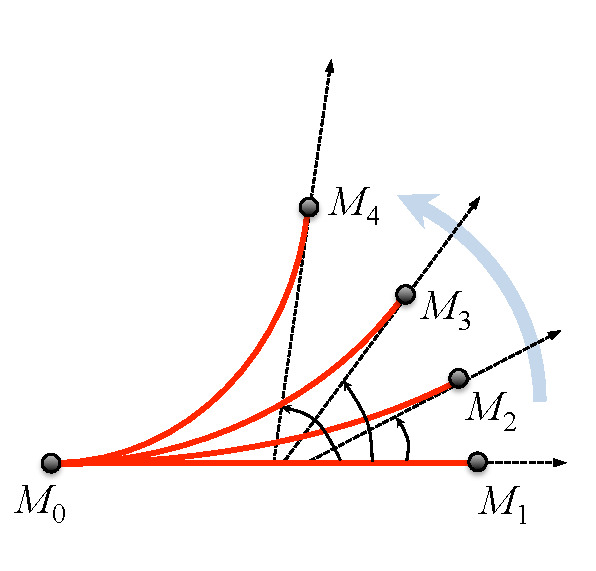
\includegraphics{./images/curves/c101.pdf}}}

				\vspace{-1em}{{\b 长度相同的曲线,切线

				转角越大弯曲程度越大}}
			\end{center}
		\column{.5\textwidth}
	\end{columns}
\end{frame}

\begin{frame}{曲率}
	\linespread{1.2}
	\centerline{\ba{如何刻画曲线的弯曲程度?}}

	\begin{columns}
		\column{.5\textwidth}
			\begin{center}
				\vspace{-1em}
				{\resizebox{!}{5.5cm}{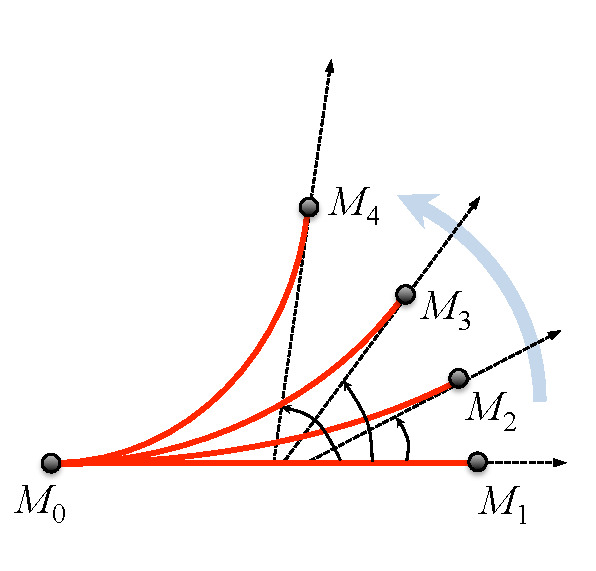
\includegraphics{./images/curves/c101.pdf}}}

				\vspace{-1em}{{\b 长度相同的曲线,切线
				
				转角越大弯曲程度越大}}	
			\end{center}
		\column{.5\textwidth}
			\begin{center}			
				\vspace{-1em}
				{\resizebox{!}{5.5cm}{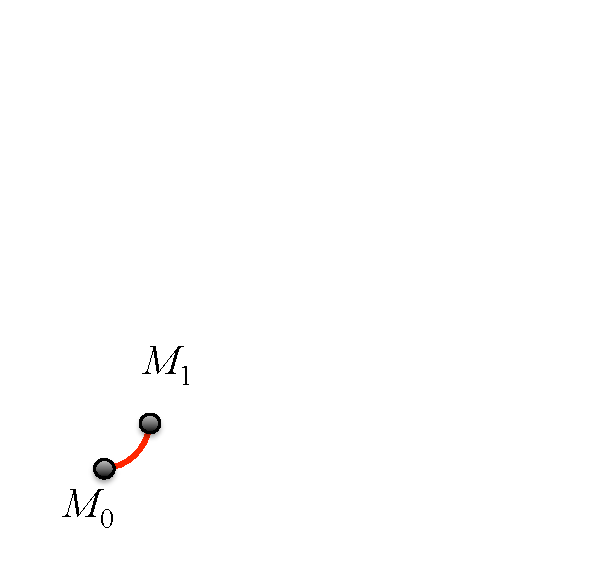
\includegraphics{./images/curves/c208.pdf}}}
				
				\vspace{-1em}{\color{white} 切线转角相同的曲线,

				弧长越短弯曲程度越大}
			\end{center}
	\end{columns}
\end{frame}

\begin{frame}{曲率}
	\linespread{1.2}
	\centerline{\ba{如何刻画曲线的弯曲程度?}}

	\begin{columns}
		\column{.5\textwidth}
			\begin{center}
				\vspace{-1em}
				{\resizebox{!}{5.5cm}{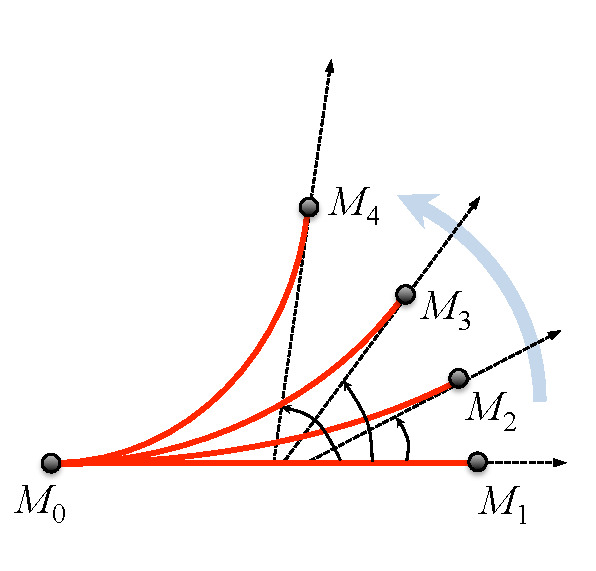
\includegraphics{./images/curves/c101.pdf}}}

				\vspace{-1em}{{\b 长度相同的曲线,切线

				转角越大弯曲程度越大}}
			\end{center}
		\column{.5\textwidth}
			\begin{center}
				\vspace{-1em}
				{\resizebox{!}{5.5cm}{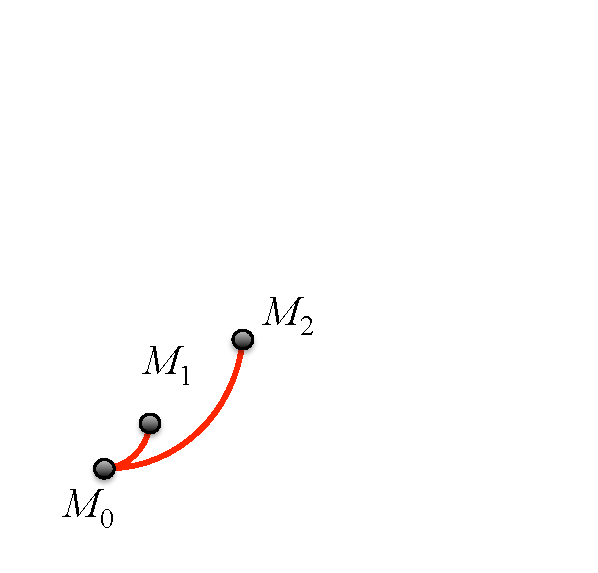
\includegraphics{./images/curves/c207.pdf}}}
				
				\vspace{-1em}{\color{white} 切线转角相同的曲线,

				弧长越短弯曲程度越大}
			\end{center}
	\end{columns}
\end{frame}

\begin{frame}{曲率}
	\linespread{1.2}
	\centerline{\ba{如何刻画曲线的弯曲程度?}}

	\begin{columns}
		\column{.5\textwidth}
			\begin{center}
				\vspace{-1em}
				{\resizebox{!}{5.5cm}{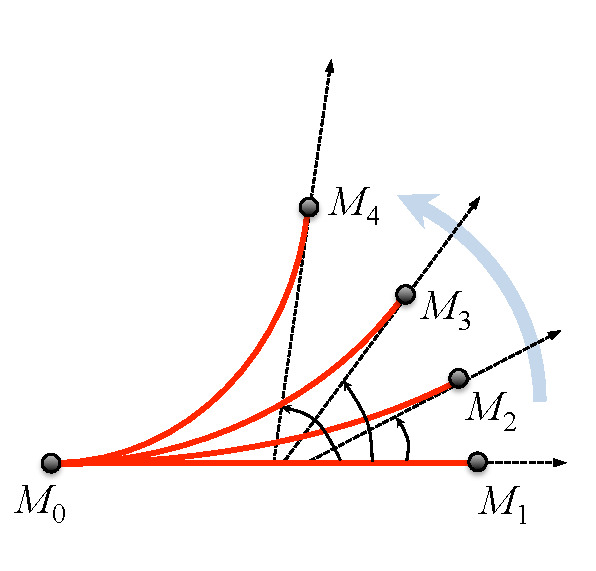
\includegraphics{./images/curves/c101.pdf}}}

				\vspace{-1em}{{\b 长度相同的曲线,切线

				转角越大弯曲程度越大}}
			\end{center}
		\column{.5\textwidth}
			\begin{center}
				\vspace{-1em}
				{\resizebox{!}{5.5cm}{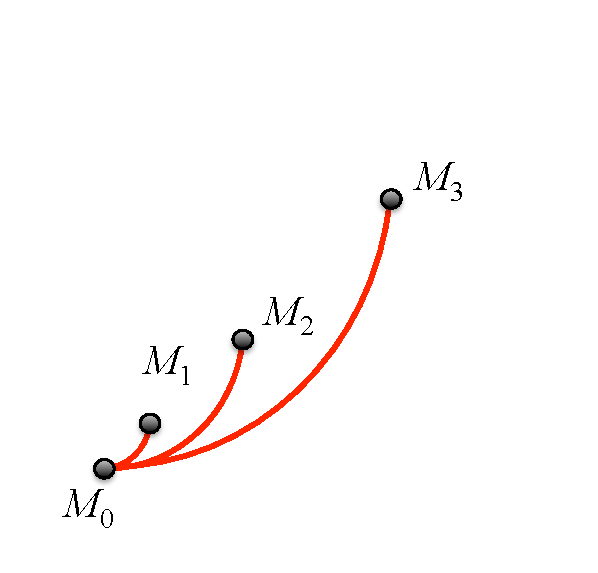
\includegraphics{./images/curves/c206.pdf}}}
				
				\vspace{-1em}{\color{white} 切线转角相同的曲线,

				弧长越短弯曲程度越大}
			\end{center}
	\end{columns}
\end{frame}

\begin{frame}{曲率}
	\linespread{1.2}
	\centerline{\ba{如何刻画曲线的弯曲程度?}}

	\begin{columns}
		\column{.5\textwidth}
			\begin{center}
				\vspace{-1em}
				{\resizebox{!}{5.5cm}{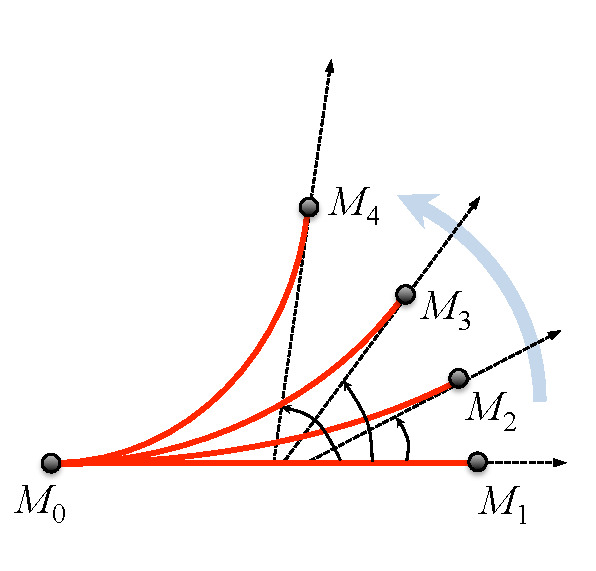
\includegraphics{./images/curves/c101.pdf}}}

				\vspace{-1em}{{\b 长度相同的曲线,切线

				转角越大弯曲程度越大}}
			\end{center}
		\column{.5\textwidth}
			\begin{center}
				\vspace{-1em}
				{\resizebox{!}{5.5cm}{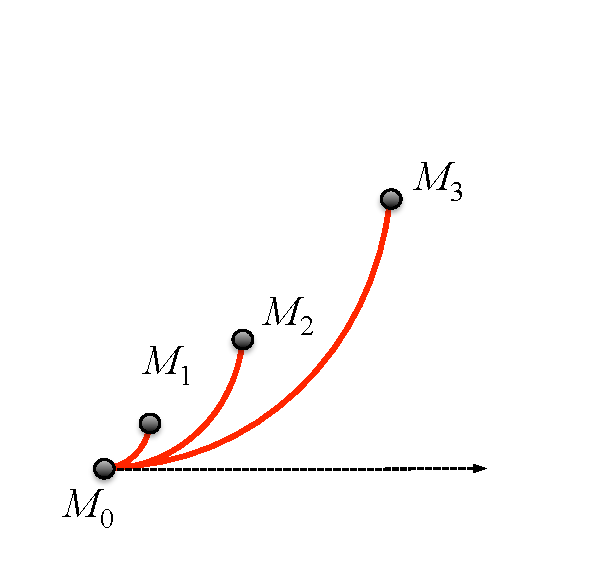
\includegraphics{./images/curves/c205.pdf}}}
				
				\vspace{-1em}{\color{white} 切线转角相同的曲线,

				弧长越短弯曲程度越大}
			\end{center}
	\end{columns}
\end{frame}

\begin{frame}{曲率}
	\linespread{1.2}
	\centerline{\ba{如何刻画曲线的弯曲程度?}}

	\begin{columns}
		\column{.5\textwidth}
			\begin{center}
				\vspace{-1em}
				{\resizebox{!}{5.5cm}{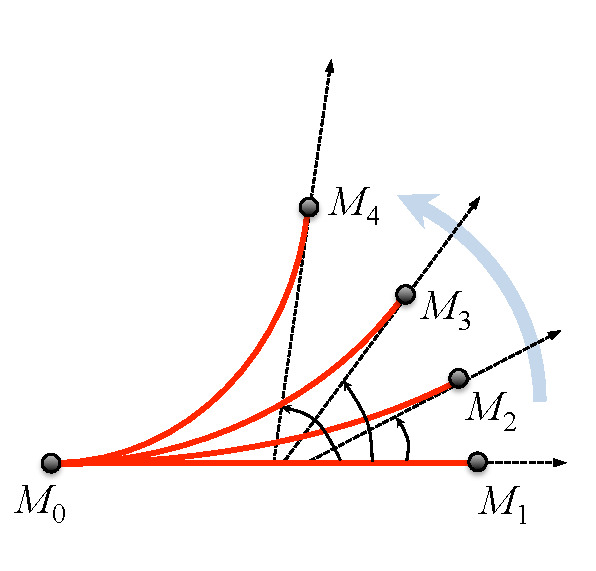
\includegraphics{./images/curves/c101.pdf}}}

				\vspace{-1em}{{\b 长度相同的曲线,切线

				转角越大弯曲程度越大}}
			\end{center}
		\column{.5\textwidth}
			\begin{center}
				\vspace{-1em}
				{\resizebox{!}{5.5cm}{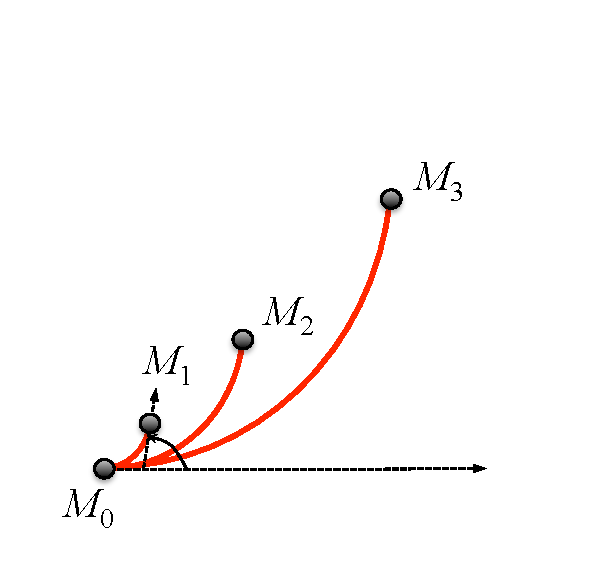
\includegraphics{./images/curves/c204.pdf}}}
				
				\vspace{-1em}{\color{white} 切线转角相同的曲线,

				弧长越短弯曲程度越大}
			\end{center}
	\end{columns}
\end{frame}

\begin{frame}{曲率}
	\linespread{1.2}
	\centerline{\ba{如何刻画曲线的弯曲程度?}}

	\begin{columns}
		\column{.5\textwidth}
			\begin{center}
				\vspace{-1em}
				{\resizebox{!}{5.5cm}{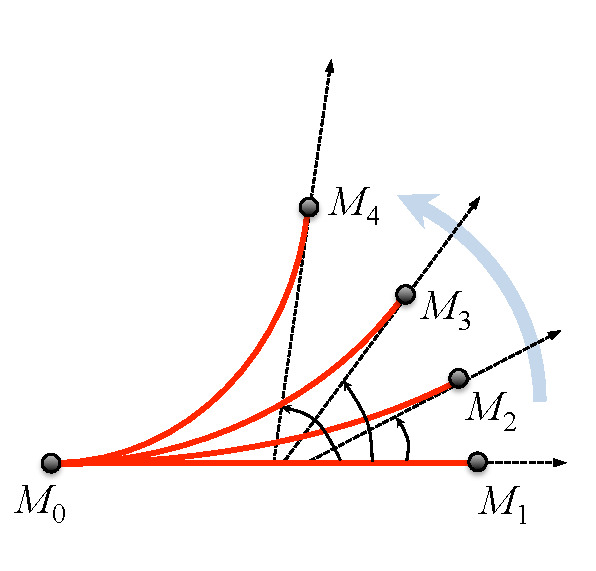
\includegraphics{./images/curves/c101.pdf}}}

				\vspace{-1em}{{\b 长度相同的曲线,切线

				转角越大弯曲程度越大}}
			\end{center}
		\column{.5\textwidth}
			\begin{center}
				\vspace{-1em}
				{\resizebox{!}{5.5cm}{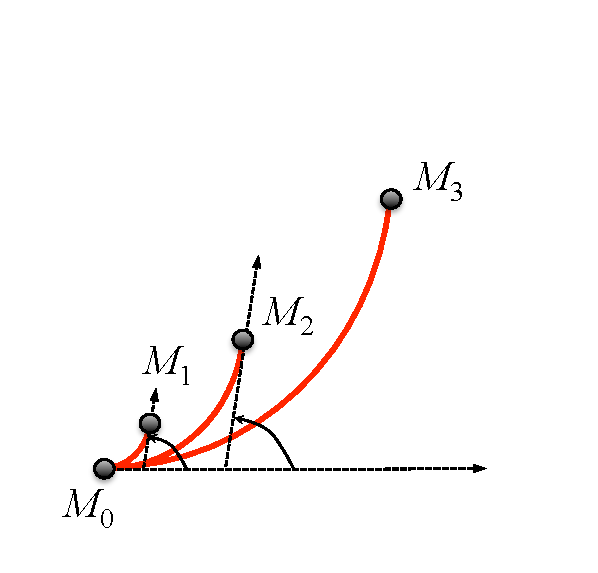
\includegraphics{./images/curves/c203.pdf}}}
				
				\vspace{-1em}{\color{white} 切线转角相同的曲线,

				弧长越短弯曲程度越大}
			\end{center}
	\end{columns}
\end{frame}

\begin{frame}{曲率}
	\linespread{1.2}
	\centerline{\ba{如何刻画曲线的弯曲程度?}}

	\begin{columns}
		\column{.5\textwidth}
			\begin{center}
				\vspace{-1em}
				{\resizebox{!}{5.5cm}{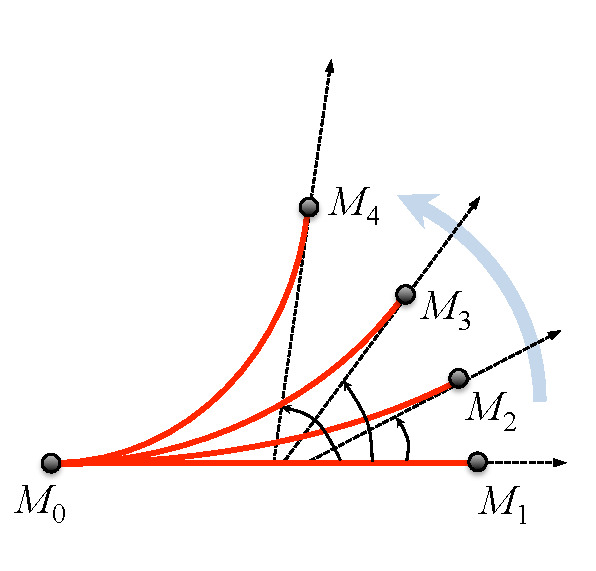
\includegraphics{./images/curves/c101.pdf}}}

				\vspace{-1em}{{\b 长度相同的曲线,切线

				转角越大弯曲程度越大}}
			\end{center}
		\column{.5\textwidth}
			\begin{center}
				\vspace{-1em}
				{\resizebox{!}{5.5cm}{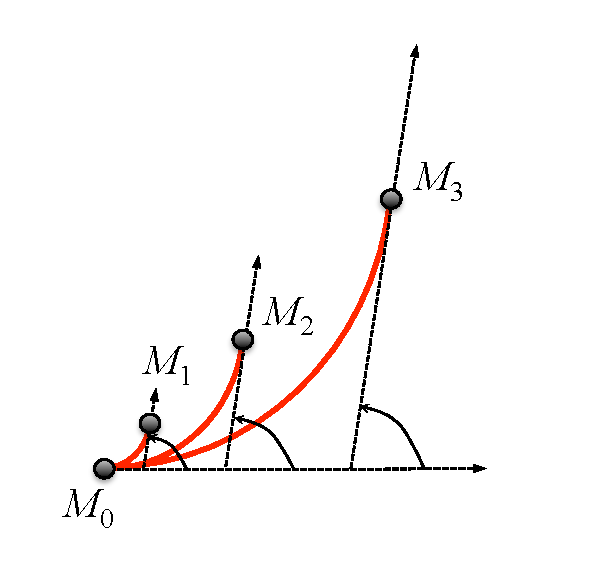
\includegraphics{./images/curves/c202.pdf}}}
				
				\vspace{-1em}{\color{white} 切线转角相同的曲线,

				弧长越短弯曲程度越大}
			\end{center}
	\end{columns}
\end{frame}

\begin{frame}{曲率}
	\linespread{1.2}
	\centerline{\ba{如何刻画曲线的弯曲程度?}}

	\begin{columns}
		\column{.5\textwidth}
			\begin{center}
				\vspace{-1em}
				{\resizebox{!}{5.5cm}{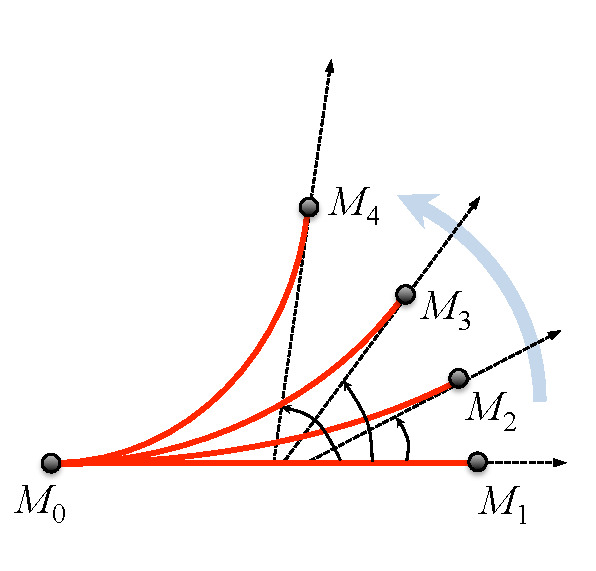
\includegraphics{./images/curves/c101.pdf}}}

				\vspace{-1em}{{\b 长度相同的曲线,切线

				转角越大弯曲程度越大}}
			\end{center}
		\column{.5\textwidth}
			\begin{center}
				\vspace{-1em}
				{\resizebox{!}{5.5cm}{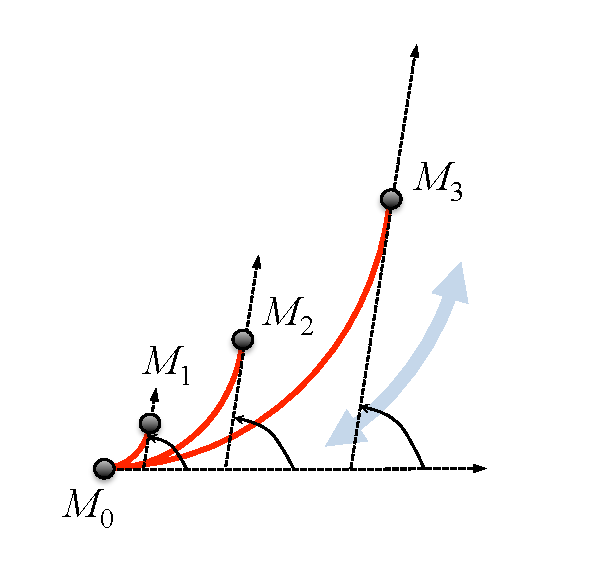
\includegraphics{./images/curves/c201.pdf}}}
				
				\vspace{-1em}{\b 切线转角相同的曲线,

				弧长越短弯曲程度越大}
			\end{center}
	\end{columns}
\end{frame}

% \begin{frame}{曲率}
% 	\linespread{1.2}
% 	\centerline{\ba{如何刻画曲线的弯曲程度?}}
% 
% 	\begin{columns}
% 		\column{.5\textwidth}
% 			\begin{center}
% 				\vspace{-1em}
% 				{\resizebox{!}{5.5cm}{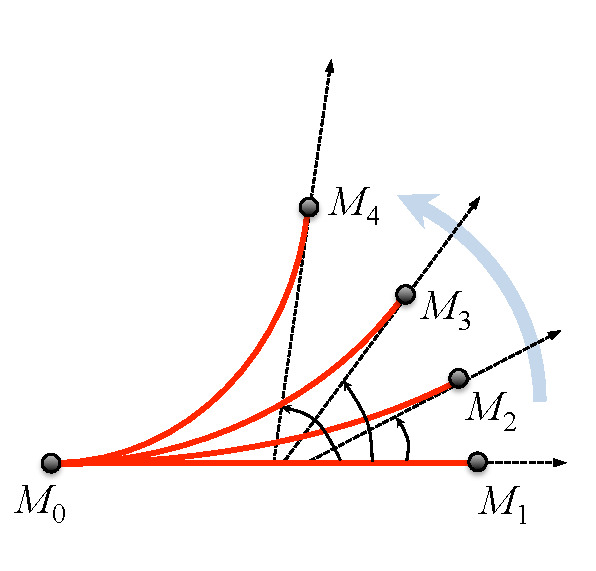
\includegraphics{./images/curves/c101.pdf}}}
% 
% 				\vspace{-1em}{{\b 长度相同的曲线,切线
% 
% 				转角越大弯曲程度越大}}
% 			\end{center}
% 		\column{.5\textwidth}
% 			\begin{center}
% 				\vspace{-1em}
% 				{\resizebox{!}{5.5cm}{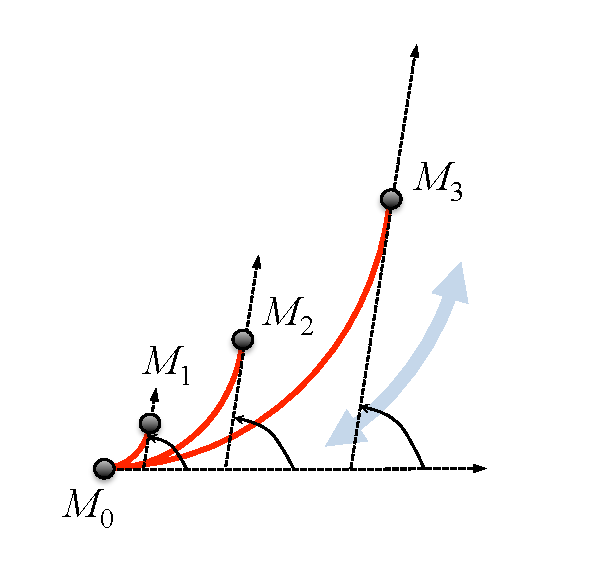
\includegraphics{./images/curves/c201.pdf}}}
% 				
% 				\vspace{-1em}{\b 切线转角相同的曲线,
% 
% 				弧长越短弯曲程度越大}
% 			\end{center}
% 	\end{columns}
% \end{frame}

%=================================================

\begin{frame}{曲率}
	\linespread{1.2}
	\centerline{\ba{如何刻画曲线的弯曲程度?}}
	\pause
	\begin{columns}
		\column{.5\textwidth}
			\begin{center}
				\vspace{-1em}
				{\resizebox{!}{5.5cm}{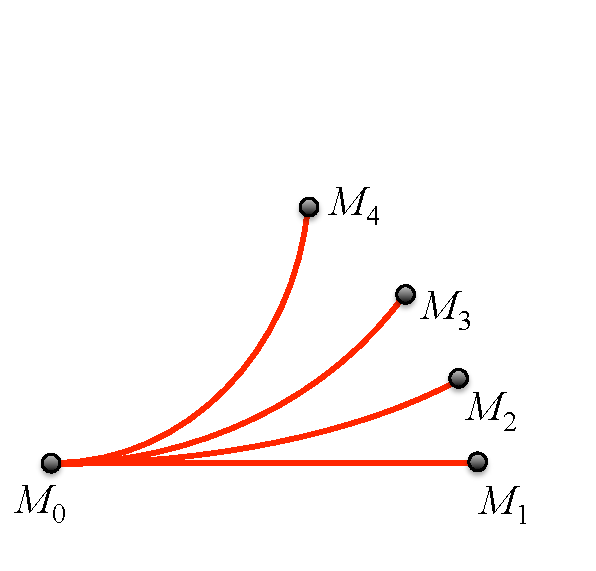
\includegraphics{./images/curves/c106.pdf}}}\pause
				
				\vspace{-5.5cm}
				\resizebox{!}{5.6cm}{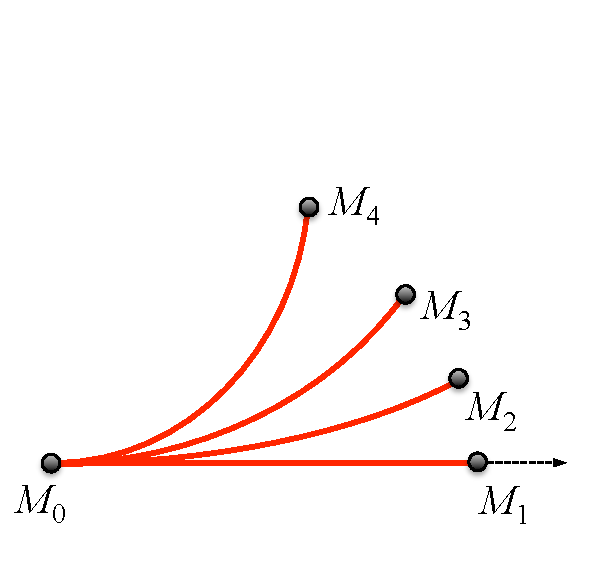
\includegraphics{./images/curves/c105.pdf}}\pause
				
				\vspace{-5.6cm}{\resizebox{!}{5.5cm}{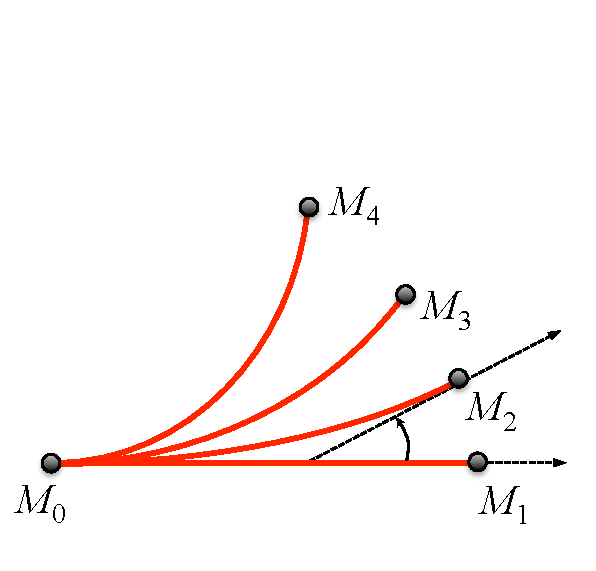
\includegraphics{./images/curves/c104.pdf}}}
% 				\only<5>{\resizebox{!}{5.5cm}{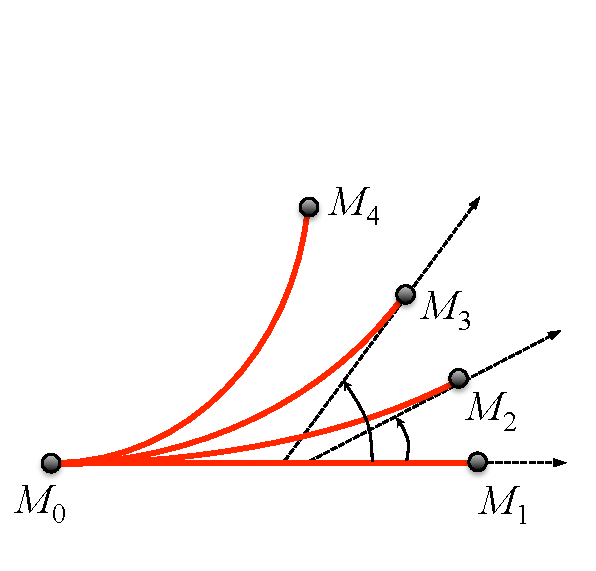
\includegraphics{./images/curves/c103.pdf}}}
% 				\only<6>{\resizebox{!}{5.5cm}{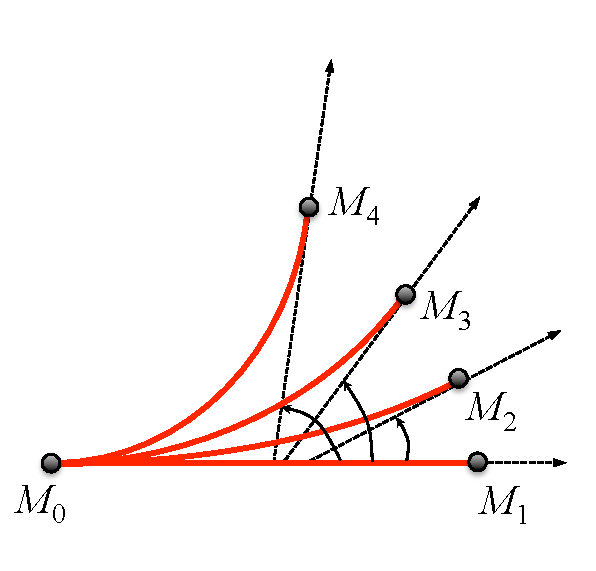
\includegraphics{./images/curves/c102.pdf}}}
% 				\only<7-17>{\resizebox{!}{5.5cm}{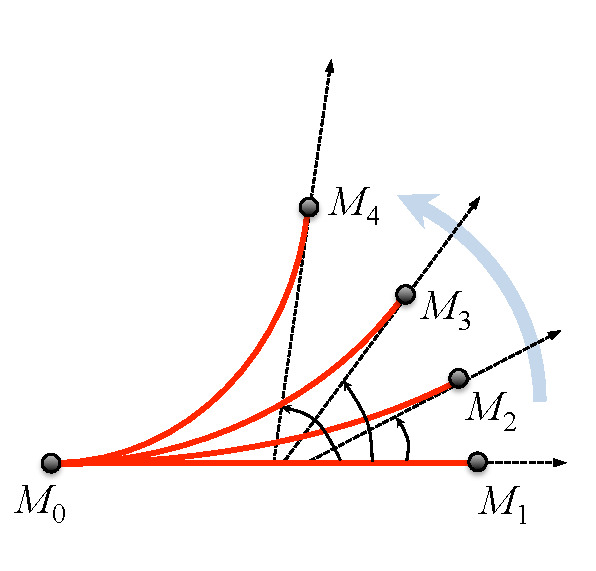
\includegraphics{./images/curves/c101.pdf}}}
% 				\only<2>{\resizebox{!}{5.5cm}{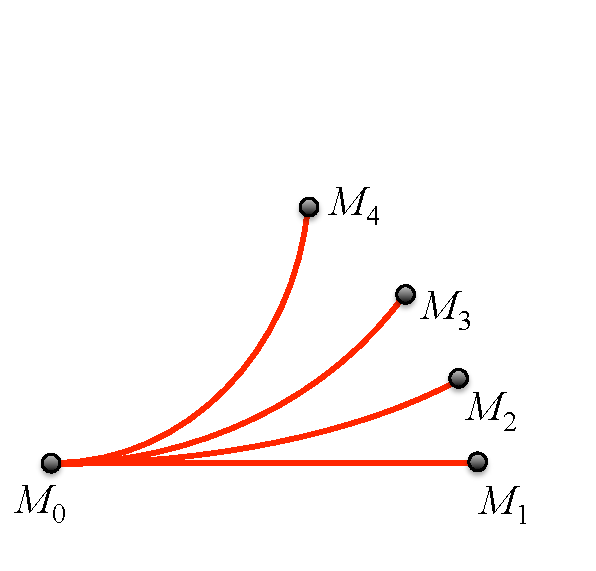
\includegraphics{./images/curves/c106.pdf}}}
% 				\only<3>{\resizebox{!}{5.5cm}{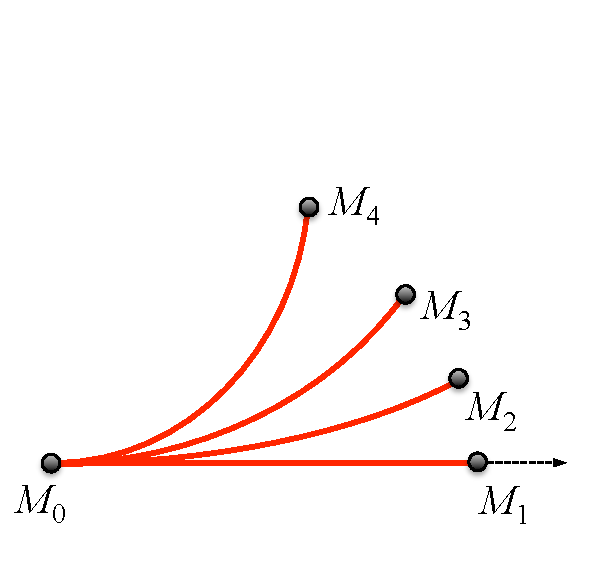
\includegraphics{./images/curves/c105.pdf}}}
% 				\only<4>{\resizebox{!}{5.5cm}{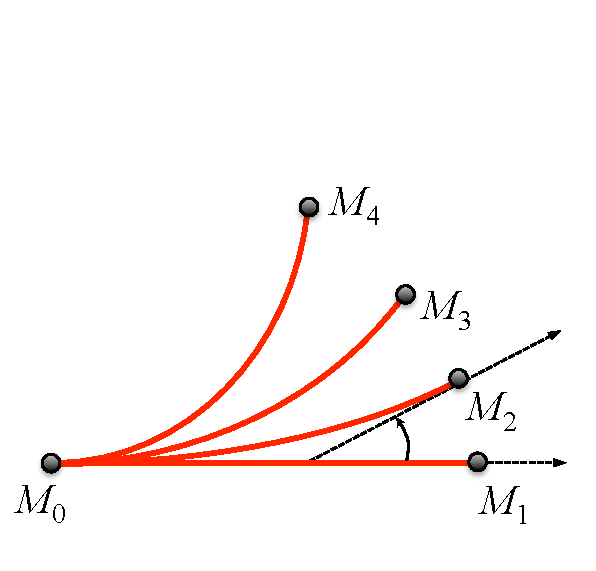
\includegraphics{./images/curves/c104.pdf}}}
% 				\only<5>{\resizebox{!}{5.5cm}{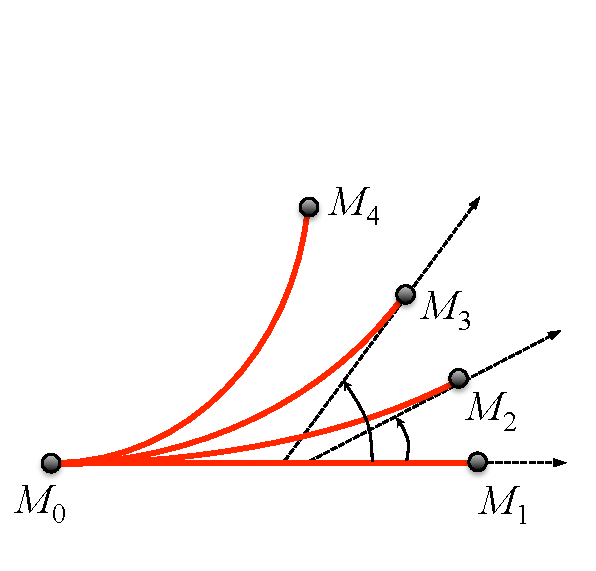
\includegraphics{./images/curves/c103.pdf}}}
% 				\only<6>{\resizebox{!}{5.5cm}{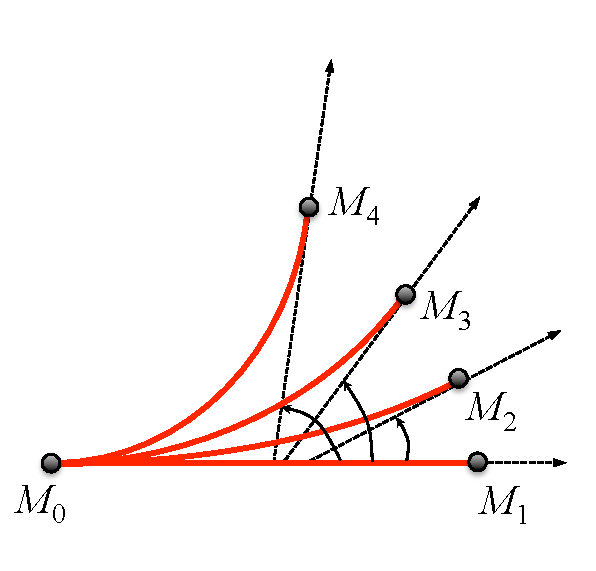
\includegraphics{./images/curves/c102.pdf}}}
% 				\only<7-17>{\resizebox{!}{5.5cm}{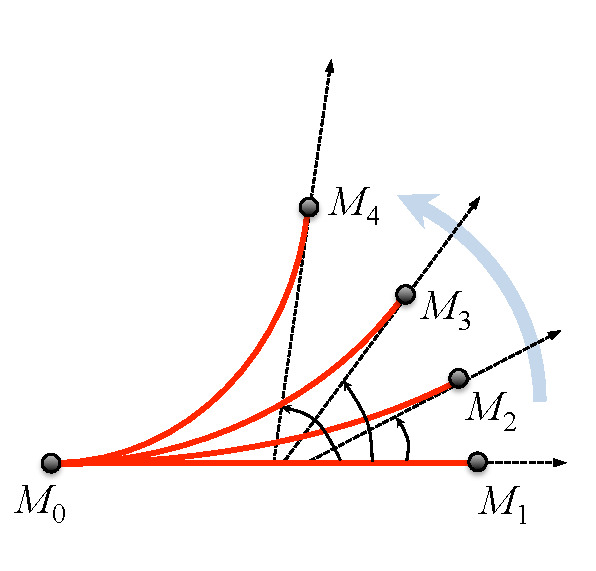
\includegraphics{./images/curves/c101.pdf}}}

				\vspace{-1em}\pause {\b 长度相同的曲线,切线

				转角越大弯曲程度越大}
			\end{center}
		\column{.5\textwidth}
			\begin{center}
				\vspace{-1em}
				\only<9>{\resizebox{!}{5.5cm}{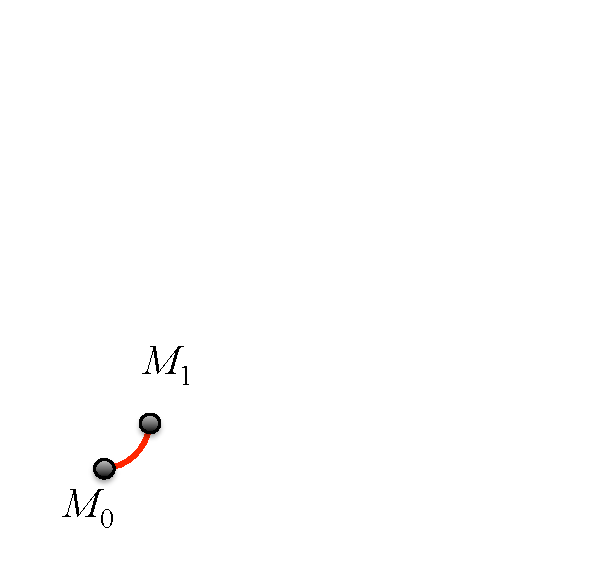
\includegraphics{./images/curves/c208.pdf}}}
				\only<10>{\resizebox{!}{5.5cm}{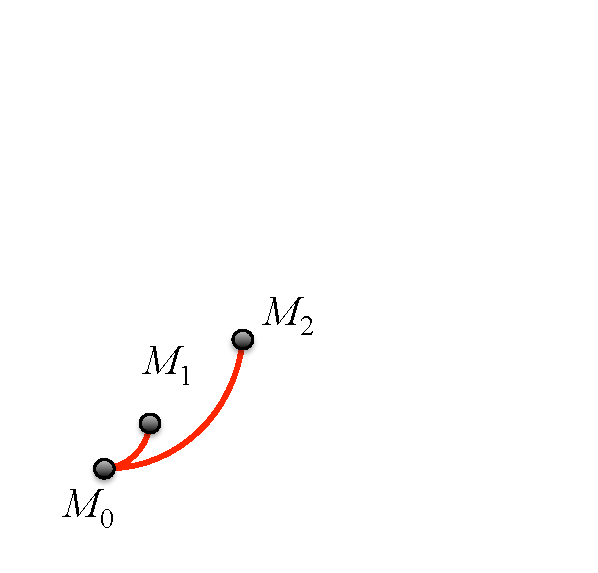
\includegraphics{./images/curves/c207.pdf}}}
				\only<11>{\resizebox{!}{5.5cm}{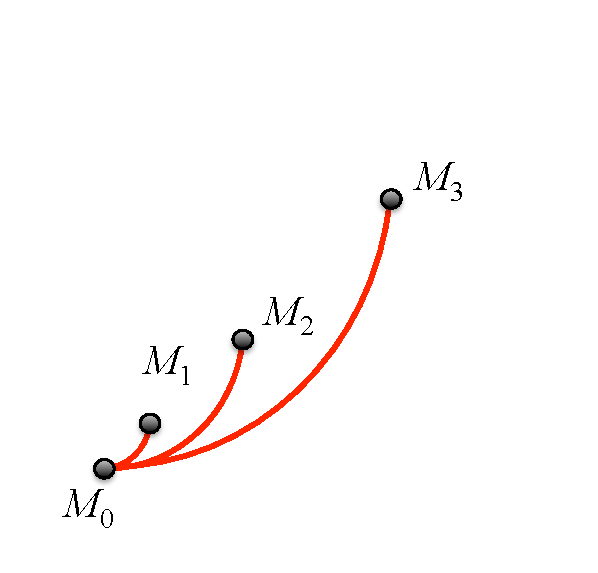
\includegraphics{./images/curves/c206.pdf}}}
				\only<12>{\resizebox{!}{5.5cm}{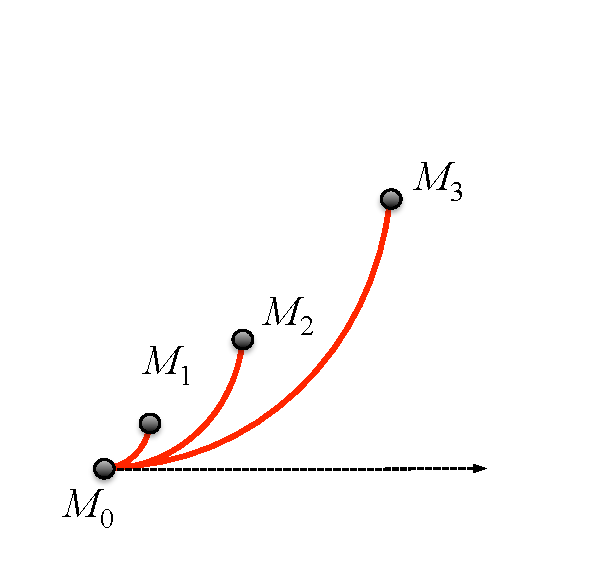
\includegraphics{./images/curves/c205.pdf}}}
				\only<13>{\resizebox{!}{5.5cm}{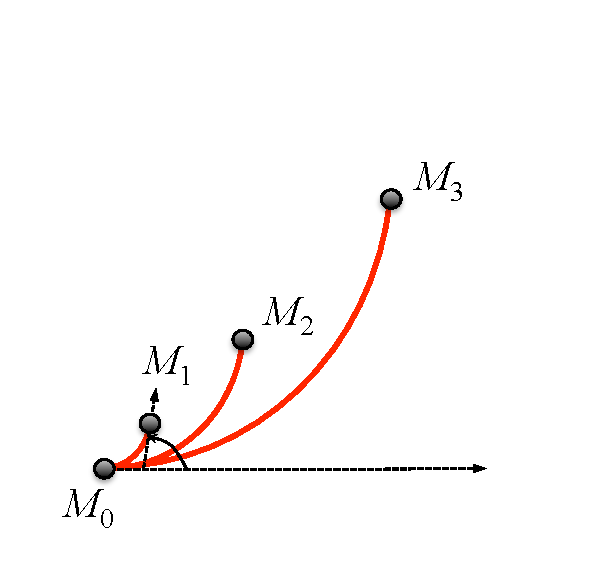
\includegraphics{./images/curves/c204.pdf}}}
				\only<14>{\resizebox{!}{5.5cm}{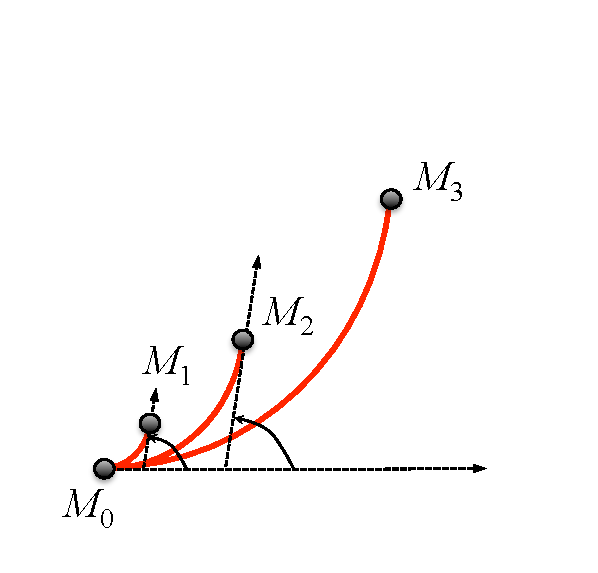
\includegraphics{./images/curves/c203.pdf}}}
				\only<15>{\resizebox{!}{5.5cm}{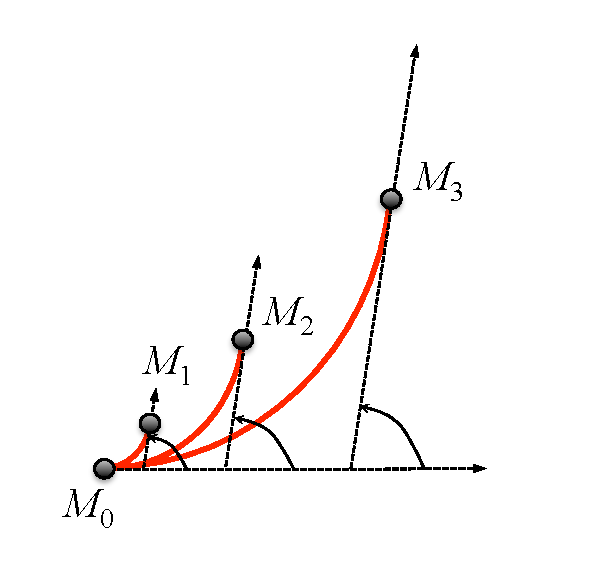
\includegraphics{./images/curves/c202.pdf}}}
				\only<16-17>{\resizebox{!}{5.5cm}{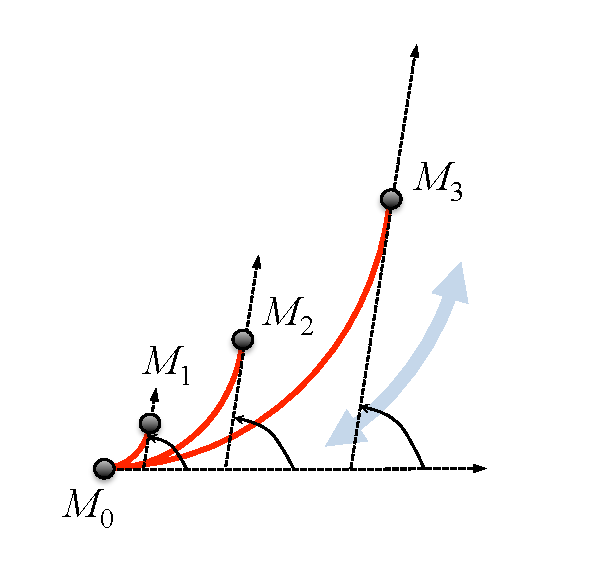
\includegraphics{./images/curves/c201.pdf}}}

				\onslide<17>
				\vspace{-1em}{\b 切线转角相同的曲线,

				弧长越短弯曲程度越大}
			\end{center}
	\end{columns}
\end{frame}

\begin{frame}{曲率}
	\linespread{1.2}
	\centerline{\ba{如何刻画曲线的弯曲程度?}}\pause 
	\begin{columns}
		\column{.5\textwidth}
			\begin{center}
				\vspace{-1em}
				\resizebox{!}{5.5cm}{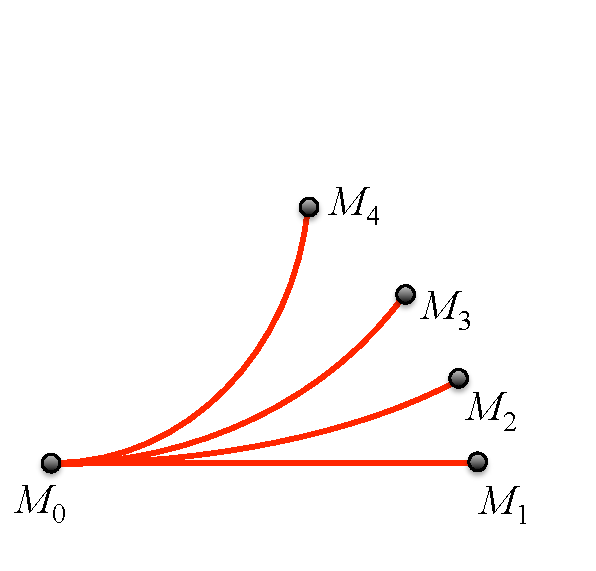
\includegraphics{./images/curves/c106.pdf}}
				
% 				\pause
				\invisible<1->{\vspace{-1em} {\b 长度相同的曲线,
				
				转角越大弯曲程度越大}}%\pause 
			\end{center}
		\column{.5\textwidth}
			\begin{center}
				\vspace{-1em}
				\invisible<1->{\resizebox{!}{5.5cm}{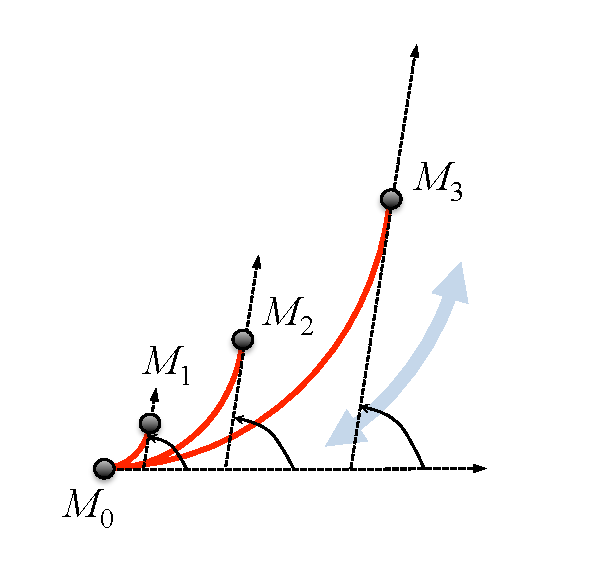
\includegraphics{./images/curves/c201.pdf}}
				
				%\pause 
				\vspace{-1em}{\b 转角相同的曲线,
				
				弧长越短弯曲程度越大}}
			\end{center}
	\end{columns}
\end{frame}

\begin{frame}{曲率}
	\linespread{1.2}
	\centerline{\ba{如何刻画曲线的弯曲程度?}}
	\begin{columns}
		\column{.5\textwidth}
			\begin{center}
				\vspace{-1em}
				\resizebox{!}{5.5cm}{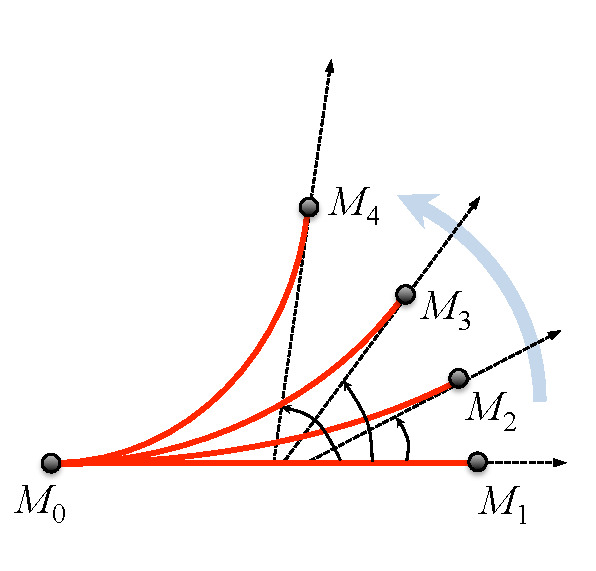
\includegraphics{./images/curves/c101.pdf}}
				
				\pause\vspace{-1em} {\b 长度相同的曲线,
				
				转角越大弯曲程度越大}%\pause 
			\end{center}
		\column{.5\textwidth}
			\begin{center}
				\vspace{-1em}
				\invisible<1->{\resizebox{!}{5.5cm}{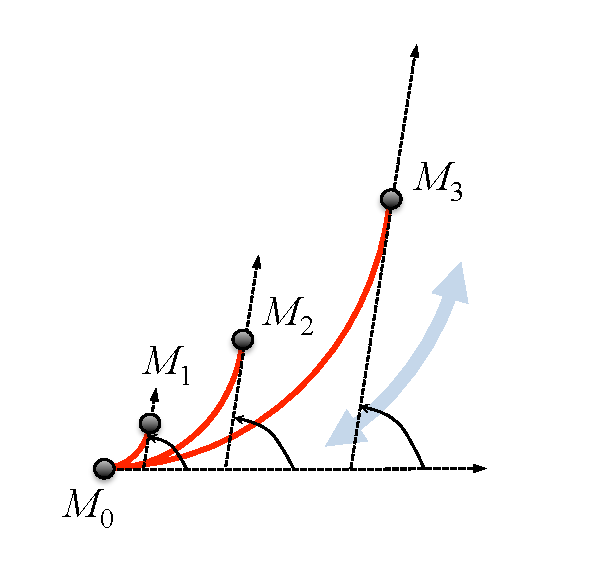
\includegraphics{./images/curves/c201.pdf}}
				
				%\pause 
				\vspace{-1em}{\b 转角相同的曲线,
				
				弧长越短弯曲程度越大}}
			\end{center}
	\end{columns}
\end{frame}

\begin{frame}{曲率}
	\linespread{1.2}
	\centerline{\ba{如何刻画曲线的弯曲程度?}}\pause 
	\begin{columns}
		\column{.5\textwidth}
			\begin{center}
				\vspace{-1em}
				\resizebox{!}{5.5cm}{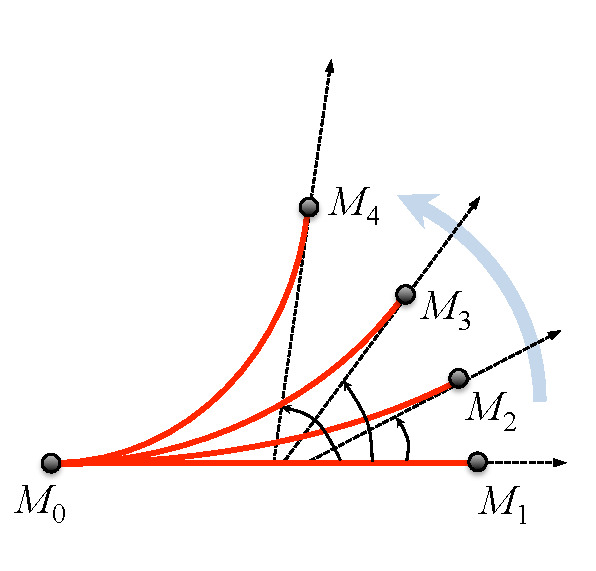
\includegraphics{./images/curves/c101.pdf}}
				
				\pause\vspace{-1em} {\b 长度相同的曲线,
				
				转角越大弯曲程度越大}\pause 
			\end{center}
		\column{.5\textwidth}
			\begin{center}
				\vspace{-1em}
				\resizebox{!}{5.5cm}{\includegraphics{./images/curves/c201.pdf}}
				
				\pause \vspace{-1em}{\b 转角相同的曲线,
				
				弧长越短弯曲程度越大}
			\end{center}
	\end{columns}
\end{frame}

\begin{frame}{曲率的定义}
	\linespread{1.5}
	\ba{曲线的弯曲程度与切线的转角成正比,弧长成反比}\pause
	
	\vspace{1em}
	\begin{columns}
		\column{.6\textwidth}
			\begin{center}
				\resizebox{!}{5cm}{\includegraphics{./images/def.pdf}}
			\end{center}
		\column{.6\textwidth}
			\pause 
			设曲线$C$在点$M_0$附近\pause 
			\begin{itemize}
			  \item 光滑\pause 
			  \item 可求长度\pause 
			\end{itemize}
			{\bb 曲线$C$在点$M_0$的曲率}
			$$\hspace{-2cm}\alert{K=\lim\limits_{\Delta s\to
				0}\left|\df{\Delta\alpha}{\Delta s}\right|\pause
				=\left|\df{d\alpha}{ds}\right|}$$
	\end{columns}
\end{frame}

\begin{frame}
	\linespread{1.2} 
	$$\alert{K=\lim\limits_{\Delta s\to
				0}\left|\df{\Delta\alpha}{\Delta s}\right|
				=\left|\df{d\alpha}{ds}\right|}$$ 
	\begin{exampleblock}{{\bf 例1}\hfill P286-例2}
		求直线上任一点处的曲率。
	\end{exampleblock}
	\pause {\bf 解:}直线上任一点处的切线就是直线本身\pause ,故其上任意两点之间的线段上
	的切线转角$\Delta\alpha=0$,\pause 从而
	$$K=\lim\limits_{\Delta s\to 0}\left|
	\df{\Delta\alpha}{\Delta s}\right|=0.$$
	\vspace{-1em}
	\begin{itemize}\pause 
	  \item \ba{$K=0$:直线不弯曲!}
	\end{itemize}
\end{frame}

\begin{frame}
	\linespread{1.2}
	\begin{exampleblock}{{\bf 例2}\hfill P286-例2}
		求半径为$R$的圆上任一点处的曲率。
	\end{exampleblock}
	\pause 
	\begin{columns}
		\column{.7\textwidth}
			\begin{center}
				\resizebox{!}{4.5cm}{\includegraphics{./images/sphere.pdf}}
			\end{center}
		\column{.3\textwidth}\pause 
			$$\alert{K=\df 1R}$$
	\end{columns}
	\begin{itemize}\pause 
	  \item \ba{圆上每一点处曲率相同}\pause 
	  \item \ba{圆的半径越小,曲率越大}
	\end{itemize}
\end{frame}

\begin{frame}{曲率的计算}
	\linespread{1.2}\pause 
	设$y=f(x)$二阶可导,则
	\alert{$$K=\lim\limits_{\Delta s\to
				0}\left|\df{\Delta\alpha}{\Delta s}\right|
				\pause =\df{|y''|}{[1+(y')^2]^{3/2}}$$}\pause 
	\begin{exampleblock}{{\bf 例3}\hfill P287-例5}
		抛物线$y=ax^2+bx+c$在哪一点的曲率最大?
	\end{exampleblock}\pause 
	\begin{itemize}
	  \item \ba{抛物线在顶点处的曲率最大}
	\end{itemize}
\end{frame}

\begin{frame}
	\linespread{1.2}
	\alert{{\bf 注:}根据不同形式的曲线方程,可以得到相应的曲率公式}\pause 
	\begin{enumerate}
	  \item 若曲线由参数方程$\left\{\begin{array}{l}
	  x=\varphi(t)\\ y=\psi(t)
	  \end{array}\right.$给出,\pause 则
	  $$\alert{K=\df{|\varphi'(t)\psi''(t)-\varphi''(t)\psi'(t)|}
		{\{[\varphi'(t)]^2+[\psi'(t)]^2\}^{3/2}}}$$\pause 
	  \item 若曲线方程为$x=g(y)$,\pause 则
		$$\alert{K=\df{|g''(y)|}{\{[1+[g'(y)]^2\}^{3/2}}}$$
	\end{enumerate}
\end{frame}

% \section{曲率圆与曲率半径}

\begin{frame}{曲率圆与曲率半径}
	\linespread{1.2} \pause 
	{\bb 曲率圆:}与已知曲线在凹侧相切,且曲率相同的圆
	
	\pause\vspace{1ex}
% 	\begin{columns}[t]
% 		\column{.6\textwidth}
			\begin{center}
				\resizebox{!}{4cm}{\includegraphics{./images/curSphere.pdf}}
			\end{center}
% 		\column{.4\textwidth}
% % 			\bigskip
% 			\uncover<5->{
% 			{\bb 二阶相切:}}
% 			
% 			\vspace{-2em}
% 			\begin{eqnarray*}
% 				\uncover<5->{\alert{f(x_0)}&\alert{=}&\alert{g(x_0),}\\
% 				\alert{f'(x_0)}&\alert{=}&\alert{g'(x_0),}\\
% 				\alert{f''(x_0)}&\alert{=}&\alert{g''(x_0).}}\\
% 			\end{eqnarray*}
% 			\vspace{-2em}
% % 			$$f^{(k)}(x_0)=g^{(k)}(x_0),\;k=0,1,2$$
% 	\end{columns}
	\pause
	\vspace{-2ex}
	\begin{block}{\bf 定理1}
		曲率圆与对应曲线二阶相切。
	\end{block}
\end{frame}

\begin{frame}
	\linespread{1.5} 
	\begin{exampleblock}{{\bf 例4}\hfill P287-例5}
		设某工件内侧的截痕为抛物线$y=ax^2+bx+c$,现要用圆形砂轮打磨其表面,
		问该如何选择砂轮的尺寸?
	\end{exampleblock}
	\pause 
	\begin{center}
		\resizebox{!}{5.5cm}{\includegraphics{./images/curlingR.pdf}}
	\end{center}
\end{frame}

\begin{frame}{曲率半径与离心力}
	\linespread{1.2}
	\begin{columns}
		\column{.6\textwidth}
			质量为$m$的质点以速度$v$通过光滑曲线上一点,所受离心力为
			$$F=\df{mv^2}{R},$$
			其中$R$为曲线在该点处的曲率半径。
		\column{.4\textwidth}
			\begin{center}
				\resizebox{!}{4.5cm}{\includegraphics{./images/flip.pdf}}
			\end{center}
	\end{columns}
	\pause
	$$\alert{R=\df{1}{K}=\lim\limits_{\Delta s\to 0}\left|\df{\Delta
	s}{\Delta\alpha}\right|}$$
\end{frame}

\begin{frame}{铁路中的缓和曲线}
	\linespread{1.2}\pause 
	\ba{为了确保列车行驶安全,连接直线和圆弧轨道的路段应该尽可能保证列车运行时所受离心力的平稳变化}\pause 
	\begin{center}
		\resizebox{!}{5.5cm}{\includegraphics{./images/releaseCurve.pdf}}
	\end{center}
\end{frame}

\begin{frame}[<+->]{小结}
	\linespread{1.5}
	\begin{enumerate}
	  \item {\bf 曲率:}切线转角关于弧长的相对变化率
	  \item {\bf 曲率的计算:}
	  \begin{itemize}
	    \item 对应于各种不同的曲线方程的曲率公式
	  \end{itemize}
	  \item {\bf 曲率圆与曲率半径:}
	  \begin{itemize}
	    \item 离心力与缓和曲线
	  \end{itemize}
	\end{enumerate}
	\begin{block}{{\bf 课后练习}\hfill}
		{\b\quad 习题5.5:5,6,7,8,11}
	\end{block}
\end{frame}

\begin{frame}
	\linespread{1.2}
	\begin{exampleblock}{{\bf 例}\hfill}
		汽车连同载重共$5000$kg,在抛物线桥面上行驶,已知桥的跨度
		$10$m,拱高$0.25$m,汽车经过桥顶时对桥的压力。
	\end{exampleblock}
\end{frame}

\begin{frame}
	\linespread{1.2}
	\begin{exampleblock}{{\bf 例}\hfill}
		飞机沿抛物线$y=\df{x^2}{4000}$(单位:m),在俯冲的最地点处
		速度为$v=400$m/s。飞行员体重$70$kg,求在俯冲的最低点处,飞行员
		对座椅的压力。
	\end{exampleblock}
\end{frame}

\begin{frame}
	\linespread{1.2}
	\begin{exampleblock}{{\bf 例}\hfill}
		椭圆$x=2\cos t,y=3\sin t$哪一点处曲率最大?
	\end{exampleblock}
\end{frame}

%=====================================
 
\begin{frame}{title}
	\linespread{1.2}
	\begin{exampleblock}{{\bf title}\hfill}
		123
	\end{exampleblock}
\end{frame}

\begin{frame}{title}
	\linespread{1.2}
	\begin{block}{{\bf title}\hfill}
		123
	\end{block}
\end{frame}